\section{Evaluation}
\label{sec:eval}
In this section, we introduce the datasets and experimental setup.
We compare our proposed models trained on semi-structured data
with models trained on only 
textual data or structured data.
~\footnote{ Data and source code: \url{http://anonymized.for.blind.review}.}

\subsection{Datasets}
In this experiment, we use synthetic opinion summarization datasets created from Yelp
~\footnote{https://www.yelp.com/dataset} and Amazon~\cite{HeM16}~\footnote{https://cseweb.ucsd.edu/~jmcauley/datasets.html} for training and
the standard human-annotated datasets of Yelp and Amazon for testing. 

\textbf{Training set.} The synthetic training datasets of existing SOTA opinion summarization approaches
are listed in \tabref{tab:database}. We produce the semi-structured
version of these datasets.

For the training sets with textual inputs, 
we extract the OAs and ISs from the 
textual inputs as semi-structured inputs. 
For training set with structured inputs, 
the structured inputs is the OAs extracted from the textual reviews.
We extract the ISs from these textual reviews.
The extracted OAs and ISs belonging to the same review compose the semi-structured 
input.

\textbf{Validation set and Test set.} 
Yelp~\cite{MeanSum19} contains $100$ validation pairs and $100$ test pairs. Each Yelp validation/test pair consists of $8$ reviews and $1$ corresponding human-written summary.
The Amazon~\cite{Copycat20} contains $28$ validation pairs and $32$ test pairs. Each Amazon pair in validation/test set is composed of $8$ reviews and $3$ reference summaries written by $3$ annotators.

\subsection{Baselines}

We evaluate different methods trained on their corresponding synthetic training data.
The brief description are shown in \tabref{tab:database}.
Besides, our proposed model BOI and MOI can be applied on transformer seq2seq model
~\cite{Transformer17}
and BART model~\cite{BART20}. Transformer seq2seq model is non-pretrained
and BART is pretrained.~\footnote{https://github.com/pytorch/fairseq}

\begin{table}[th]
	\small
	\centering
	\begin{tabular}{|m{1.15cm}<{\centering}|m{1.75cm}<{\centering}|l|}
		\hline
		\textbf{Approach} & \textbf{Input format} & \textbf{Model description}\\ 
		\hline
		Denoise\cut{\tablefootnote{Without released data or code of Denoise, we implement their approach.} } & Textual & Nosing \& denoising  ~\cite{Denoise20} \\
		\hline
		FewShot & Textual & Few-shot learning~\cite{Fewshot20}\\
		\hline
		PlanSum & Textual  & Content Planning~\cite{Plansum20}\\
		\hline
		OpiDig & Structured & OpinionDigest~\cite{OpiDig20}\\
		\hline
		\multirow{4}{*}{Ours} & \multirow{4}{*}{Semi-structured} 
		& \textbf{TransBOI}: BOI based on transformer \\
				\cline{3-3}
				& & \textbf{TransMOI}: MOI based on transformer  \\
		\cline{3-3}
		& & \textbf{BartBOI}: BOI based on BART \\
		\cline{3-3}
	& & \textbf{BartMOI}: MOI based on BART \\
		\hline
	\end{tabular}
	\caption{The input format of the synthetic training datasets and the models trained on these training set.}
	\label{tab:database}
\end{table}

\subsection{Implementation Details}
In this experiment, 
for the proposed model based on transformer seq2seq model, the optimizer is SGD, the initial learning rate is $0.1$, a momentum $\beta=0.1$ and a decay of  $\gamma=0.1$.
For the proposed model on BART,
we follow~\citet{BART20} in fine-tuning BART with
$lr=3e$-$05$ and warmup $=500$.
At test, the beam size is $5$.
The models are trained on one RTX 2080Ti GPU with 11G RAM. 
The average training time of our approachs is about $10$ hours.


\subsection{Evaluation Metrics}
In this experiment, we use four evaluation metrics.

%\textbf{Automatic Metrics.}

%\begin{itemize} 
%\item 
\textbf{ROUGE} scores (F1). It includes
%is the standard evaluation metric in summarization task,
ROUGE-1 (R-1), ROUGE-2 (R-2) and
ROUGE-L (R-L)~\cite{rouge}.


\textbf{Diversity} (Div). 
For a summary, Div is the average of BLEU scores of each sentence by considering others as reference~\cite{SelfBleu18}. 
The lower value means more diversity.

\textbf{Opinion Coverage} (OC).
We extract aspects from reference summary and 
generated summary 
by a rule-based method~\cite{aspect14}.
\footnote{It is different from MIN-MINER used in our approach,
	which avoids the bias caused by using the same aspect extraction tool in the approach and evaluation.}.
We then compute R-1 recall between aspects of reference summary and generated summary.
%\end{itemize}

\textbf{Human Evaluation.}
We randomly select $32$ Yelp test pairs 
and $32$ Amazon test pairs.
Three human annotators are asked
to score gold summary and summaries 
generated by our best model and 
the previous SOTA model PlanSum according to the consistency with multi-review and informativeness,
i.e., best (3.0), average (2.0) and worst (1.0).
%For a generated summary, we average the scores by
The score of a generated summary is the average score of annotators.
The score of a model is the average score of generated summaries.


\subsection{Results}
\label{sec:results}
In this section, we analyze the semi-structured data  and 
proposed models.

\begin{table*}[th]
	\begin{center}
		\small
		\begin{tabular}{|r|c|c|c|c|c|c|c|c|c|c|c|c|}
			\hline
			\multicolumn{3}{|c|}{\bf Approach} & \multicolumn{5}{c|}{\bf Yelp} &  \multicolumn{5}{c|}{\bf Amazon} \\
			\hline
			\textbf{Training data} & \textbf{Input format} & \textbf{Model} & R-1 & R-2 & R-L & OC & Div & R-1 & R-2 & R-L & OC & Div \\
			\hline
			\multirow{2}{*}{OpiDig} & Structured &OpiDig & 28.68 &5.00 & 25.33& 0.39 & 0.33 & 29.52 & 5.26 & 26.65 & 0.23 & 0.37 \\
			%\cline{2-12}	 
			&Semi-structured& TransMOI & 28.90 & 5.28 & 25.71 & 0.41 & 0.30 &30.02 & 5.39& 27.00 & 0.25 & 0.28\\
			\hline
			\multirow{2}{*}{FewShot}  & Textual & FewShot & 29.64 & 5.80 & 27.01 & 0.38 & 0.28 & 31.02 & 6.06 & 27.94 & 0.20 & 0.30 \\
			%\cline{2-12}	 
			& Semi-structured & TransMOI & 30.04 & 6.14 & 28.67 & 0.39 & 0.24 &31.42 & 6.09& 28.27 & 0.28 & 0.27\\
			\hline
			\multirow{2}{*}{Denoise} & Textual & Denoise& 29.75 & 5.00 & 26.88 & 0.39 & 0.27 &27.96 & 4.01 & 24.20& 0.16 & 0.42  \\
			%\cline{2-12}	 
			& Semi-structured & TransMOI & 29.94 & 5.84& 27.11 & 0.41 & 0.24 & 28.03& 4.54& 24.96 & 0.20 & 0.38 \\
			\hline
			\multirow{2}{*}{PlanSum}  & Textual & PlanSum & 31.19&6.83 &28.98 &0.38 & 0.27 & 31.29 &6.13 & 27.95 & 0.23 & 0.28\\  %\cline{2-13}
			& Semi-structured & BartMOI & \bf 32.03& \bf 6.92 & \bf 29.02 & \bf 0.41 & \bf 0.23 & \bf 31.89 & \bf 6.23 &  \bf 28.53& \bf 0.28 & \bf 0.23 \\
			\hline
		\end{tabular}
	\end{center}
	\caption{The comparison of the datasets with structured input, textual input and semi-structured input. We use TransMOI and BartMOI to train the input in semi-structured version because of the characteristics of semi-structured data.}
	\label{tab:traindata}  
\end{table*}

\begin{figure*} \centering 
	\subfigure[ROUGE-2] { \label{fig:a} 
		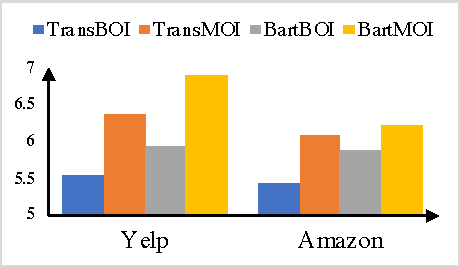
\includegraphics[width=0.6\columnwidth]{R2.pdf} 
	} 
	\subfigure[Opinion Coverage] { \label{fig:b} 
		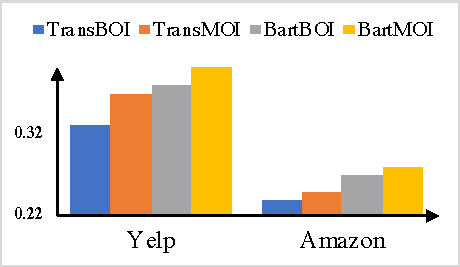
\includegraphics[width=0.6\columnwidth]{OC.pdf} 
	} 
	\subfigure[Diversity] { \label{fig:c} 
		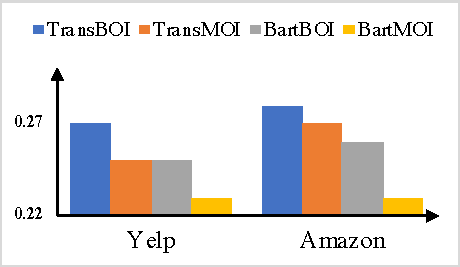
\includegraphics[width=0.6\columnwidth]{Div.pdf} 
	} 
	\caption{The evaluation of summaries generated by models trained on the semi-structured version of PlanSum data.} 
	\label{fig:acdv} 
\end{figure*} 

\textbf{Semi-structured data.}
We compare the results of the sturctured or textual inputs training on their corresponding models with the semi-structured version of these inputs training on model TransMOI or BartMOI.
%The results are listed in \tabref{tab:traindata}.

In \tabref{tab:traindata}, the synthetic training data with inputs in different formats are trained on different models since
the synthetic dataset is compatible with its model 
and performs best on its model.
As the model of PlanSum is pretrained and other models is non-pretrained,
we compare BartMOI (pretrained) trained on semi-structured data
with PlanSum and compare TransMOI (non-pretrained) trained on semi-structured data with other approaches, to be fair.

As shown in \tabref{tab:traindata}, the ROUGE, OC and Div score are improved after convering structured input into semi-structured input, which shows the ISs in semi-structured data help model capture important information that the structured data may lose.
The semi-structured data 
is better than its textual version in terms of ROUGE, OC and Div,
showing that semi-structured data
can highlight the aspects and opinions better.
Thus,
the semi-structured data is more effective than structured or textual data on opinion summarization task.

\begin{table}[th]
	\begin{center}
		\small
		\begin{tabular}{|m{0.5cm}|m{7.2cm}|}	
			\hline
			BOI & the \textbf{food} is good and the \textcolor{red}{meal} is great .
			The famliy \textcolor{red}{atmosphere} is great . The \textbf{price} and \textbf{protions} are amazing . \\
			\hline
			MOI &the \textbf{food} is delicious and can be \textbf{taken out} . the \textbf{price} is amazing and the \textbf{portions} are very generous . the \textbf{kabob} is wonderful . \\
			
			\hline
		\end{tabular}
	\end{center}
	\caption{The summaris of \tabref{tab:previous_data} generated by BART-based models trained on semi-structured version of PlanSum data.
		%Bold words can match aspects of reference and 
		Red words cannot math reference.
	}\label{tab:exp}  
\end{table}

\textbf{Proposed models.}
As shown in \figref{fig:acdv}, MOI gets better performance than BOI on all evaluation metrics. 
This shows that
MOI is a better way to expand important OAs to sentences and summarize ISs. 
MOI uses two encoders to encode OAs and ISs by different pipelines
at the same time. BOI encodes the concatenation of OAs and ISs by a single encoder. 
However, BOI equally deals with OAs and ISs,
and interferes with the model's understanding of OAs and ISs. 
As shown in \tabref{tab:exp},
BOI still matchs some noisy aspects of reference summary, such as ``meal'' and ``atmosphere''.
BOI is also unable to summarize ISs well.
BOI cannot capture the information about ``take out''.
Besides, because of directly using OAs as input, the OC scores of different models are similar. The BART-based models have better performance because BART is pretrained model.


\textbf{Human evaluation.} 
We use human evaluation to compare our best model (BartMOI) with the best approach on opinion summarization (PlanSum).
The better human evaluation score means the summaries
are more informative and consistent with input.
As shown in \tabref{tab:human}, 
Gold summary get best score.
The summaries generated by BartMOI trained on semi-structured data
performs better than PlanSum trained on textual data.


\begin{table}[th]
	\centering
	\small
	\begin{tabular}{|l|c|c|c|}
		\hline 
		& Gold & PlanSum & BartMOI\\
		\hline
		Yelp & \bf{2.4} &  1.3 & 2.2\\
		Amazon &\bf{2.3} & 1.8 & 2.0 \\
		\hline
	\end{tabular}
	\caption{Human evaluation. \protect\footnotemark
	}\label{tab:human}  
\end{table}
~\footnotetext{The Kappa coefficient is $0.6$, indicating substantial agreement.}









